% !TEX program = lualatex
% ═══════════════════════════════════════════════════════════════════════
%  Chapitre 5 — L'analyse en composantes principales
%  Diaporama Beamer pour un exposé magistral (~4 heures)
%  Jérôme Soucy — MAT-2901
%
%  Compilation : lualatex main.tex   (deux passages, pour le sommaire)
%
%  Ce diaporama reprend les définitions, propositions/théorèmes (énoncés
%  seulement), exemples, figures et tableaux du chapitre 5 des notes de
%  cours. Les démonstrations ne sont PAS reproduites : chaque résultat
%  qui, dans les notes, porte une démonstration est plutôt marqué
%  « DÉMONSTRATION AU TABLEAU », avec un rappel très court de l'idée, à
%  l'intention de la personne qui présente.
%
%  Les figures sont celles du livre (../../figures/tikz/fig-acp-*.tikz).
%  Section 3 : lien vers l'application interactive des manchots, à
%  présenter en classe.
% ═══════════════════════════════════════════════════════════════════════
\documentclass[aspectratio=169, 11pt]{beamer}
% ═══════════════════════════════════════════════════════════════════════
%  preambule.tex — Réglages, couleurs et raccourcis communs du diaporama
%  du chapitre 5 (« L'analyse en composantes principales »).
%  Ce fichier est autonome : il ne dépend d'aucun fichier du livre.
% ═══════════════════════════════════════════════════════════════════════

% ── Encodage, langue, polices (lualatex, comme le livre) ───────────────
\usepackage{fontspec}
\usepackage[french]{babel}

\setmainfont{TeX Gyre Termes}
\IfFontExistsTF{Fira Sans}
  {\setsansfont{Fira Sans}[Scale=MatchLowercase]}
  {\setsansfont{TeX Gyre Heros}[Scale=MatchLowercase]}
\usefonttheme{professionalfonts}
\renewcommand{\familydefault}{\sfdefault}

\usepackage{amsmath}   % avant unicode-math (sinon \underbrace est cassé)
\usepackage{mathtools}
\usepackage{unicode-math}
\IfFontExistsTF{NewCMMath-Book.otf}
  {\setmathfont{NewCMMath-Book}}
  {\setmathfont{Latin Modern Math}}

\usepackage{booktabs}
\usepackage{array}
\usepackage{graphicx}
\usepackage{adjustbox}
\usepackage{siunitx}
\sisetup{output-decimal-marker = {,}, exponent-product = \times,
         group-separator = {\,}, group-minimum-digits = 4}
\usepackage[skins,breakable]{tcolorbox}
\usepackage{tikz}
\usetikzlibrary{calc, arrows.meta, angles, quotes, patterns, positioning,
                decorations.markings, backgrounds, fit, shapes.geometric}

% ── Palette (identique à celle du livre, livrejs.cls) ──────────────────
\definecolor{sectioncolor}{RGB}{28, 63, 110}   % bleu foncé — titres
\definecolor{thmboxbg}{RGB}{228, 238, 252}     % bleu pâle — énoncés
\definecolor{coveraccent}{RGB}{196, 142, 58}   % or chaud — accent
\definecolor{secboxbg}{RGB}{253, 240, 219}     % ocre pâle — « Pour la classe »
\definecolor{steelblue4}{HTML}{36648B}         % figures : objet de départ
\definecolor{firebrick3}{HTML}{CD3333}         % figures : objet image
\definecolor{demobg}{RGB}{247, 247, 247}       % fond neutre — « au tableau »
\definecolor{bgpage}{RGB}{253, 253, 252}       % fond de diapositive, légèrement chaud

% ── Thème beamer : sobre, cohérent avec le livre ────────────────────────
\usecolortheme{default}
\setbeamercolor{palette primary}{bg=sectioncolor, fg=white}
\setbeamercolor{palette secondary}{bg=sectioncolor, fg=white}
\setbeamercolor{palette tertiary}{bg=sectioncolor, fg=white}
\setbeamercolor{title}{fg=sectioncolor}
\setbeamercolor{frametitle}{bg=sectioncolor, fg=white}
\setbeamercolor{structure}{fg=sectioncolor}
\setbeamercolor{section in toc}{fg=sectioncolor}
\setbeamercolor{subsection in toc}{fg=black}
\setbeamercolor{background canvas}{bg=bgpage}
\setbeamercolor{footline}{fg=gray, bg=bgpage}
\setbeamercolor{block title}{bg=sectioncolor, fg=white}
\setbeamercolor{block body}{bg=thmboxbg, fg=black}
\setbeamercolor{item}{fg=sectioncolor}
\setbeamercolor{itemize item}{fg=coveraccent}
\setbeamercolor{itemize subitem}{fg=sectioncolor}
\setbeamertemplate{itemize item}{\raise0.3ex\hbox{\small$\blacktriangleright$}}
\setbeamertemplate{itemize subitem}{\raise0.3ex\hbox{\footnotesize$\bullet$}}
\setbeamertemplate{navigation symbols}{}
\setbeamerfont{frametitle}{series=\bfseries}
\setbeamertemplate{frametitle}{%
  \vskip-1ex
  \begin{beamercolorbox}[wd=\paperwidth,ht=3.8ex,dp=1.3ex,leftskip=1em,rightskip=1em]{frametitle}
    \bfseries\strut\insertframetitle
  \end{beamercolorbox}
  \vskip3pt
}
\setbeamertemplate{footline}{%
  \leavevmode
  \hbox{\begin{beamercolorbox}[wd=\paperwidth,ht=2.4ex,dp=1ex,leftskip=1em,rightskip=1em]{footline}
    {\scriptsize\color{gray}Chapitre 5 --- L'analyse en composantes principales
    \hfill \insertshorttitle{} \hfill \insertframenumber/\inserttotalframenumber}
  \end{beamercolorbox}}%
}
\setbeamertemplate{blocks}[rounded][shadow=false]
\setbeamertemplate{section in toc}{%
  \inserttocsectionnumber.~\inserttocsection\par\vskip0.15em}

% ── Page de section : diapositive de transition ────────────────────────
\AtBeginSection[]{%
  \begin{frame}[plain,c]
    \begin{center}
      {\color{coveraccent}\rule{0.25\textwidth}{1.2pt}}\\[10pt]
      {\usebeamerfont{frametitle}\usebeamercolor[fg]{title}%
       \Large\bfseries\color{sectioncolor}\insertsectionhead}\\[10pt]
      {\color{sectioncolor}\rule{0.45\textwidth}{0.5pt}}
    \end{center}
  \end{frame}
}
\AtBeginSubsection[]{%
  \begin{frame}[plain,c]
    \begin{center}
      {\large\color{gray}\insertsectionhead}\\[4pt]
      {\Large\bfseries\color{coveraccent}\insertsubsectionhead}
    \end{center}
  \end{frame}
}

% ── Raccourcis mathématiques repris du livre (autonomes) ────────────────
\newcommand{\Plan}{\Pi}
\newcommand{\Transf}{\mathcal{T}}
\newcommand{\Aff}{\mathcal{A}}
\newcommand{\Sim}{\mathcal{S}}
\newcommand{\Iso}{\mathcal{I}}
\newcommand{\mat}[4]{\begin{pmatrix}#1 & #2\\ #3 & #4\end{pmatrix}}
\newcommand{\col}[2]{\begin{pmatrix}#1\\ #2\end{pmatrix}}
\newcommand{\coliii}[3]{\begin{pmatrix}#1\\ #2\\ #3\end{pmatrix}}
\newcommand{\norme}[1]{\lVert #1 \rVert}
\newcommand{\Aire}{\operatorname{Aire}}
\newcommand{\dete}{\operatorname{det}}
\renewcommand{\vec}[1]{\mathbf{#1}}
\DeclareMathOperator{\R}{\mathbb{R}}
\DeclareMathOperator{\Rs}{\mathbb{R}^{\star}}
\newcommand{\intff}[2]{\mathopen{[}{#1},{#2}\mathclose{]}}
\newcommand{\intoo}[2]{\mathopen{]}{#1},{#2}\mathclose{[}}
\newcommand{\defi}[1]{{\color{coveraccent}#1}}
\newcommand{\intfo}[2]{\mathopen{[}{#1},{#2}\mathclose{[}}
\DeclareMathOperator{\N}{\mathbb{N}}
\DeclareMathOperator{\Ns}{\mathbb{N}^{\star}}
\DeclareMathOperator{\Q}{\mathbb{Q}}

% ── Raccourcis propres au chapitre 2 (identiques à macros-livre.tex) ────
\newcommand{\dE}{d_E}                         % distance euclidienne
\newcommand{\dT}{d_T}                         % taxi-distance (Manhattan)
\newcommand{\dHam}{d_{\mathrm{Ham}}}          % distance de Hamming
\newcommand{\dH}{d_H}                         % distance de Hausdorff
\newcommand{\boule}[2]{B(#1, #2)}             % boule ouverte
\newcommand{\Vois}[2]{#1^{\oplus #2}}         % epsilon-voisinage (Minkowski)
\newcommand{\Comp}[1]{\mathcal{K}(#1)}        % compacts non vides de E
\newcommand{\comp}[1]{\mathopen{}#1\mathclose{}^{\mathsf{c}}}

% Images bitmap (portraits, figures Python) reprises du livre.
\graphicspath{{../../figures/portraits/}{../../figures/python/}}

% ── Styles TikZ communs à toutes les figures (identiques au livre) ──────
\tikzset{
  axe/.style        = {-{Stealth[length=2mm]}, gray!70, thin},
  quadrillage/.style= {gray!22, very thin},
  fig/.style        = {fill=steelblue4!22, draw=steelblue4, thick,
                       line join=round},
  figim/.style      = {fill=firebrick3!22, draw=firebrick3, thick,
                       line join=round},
  figaux/.style     = {fill=coveraccent!22, draw=coveraccent!85!black,
                       thick, line join=round},
  pt/.style         = {circle, fill=sectioncolor, inner sep=1.1pt},
  ptim/.style       = {circle, fill=firebrick3, inner sep=1.1pt},
  fleche/.style     = {-{Stealth[length=2.4mm]}, sectioncolor, thick},
  etiq/.style       = {font=\scriptsize, inner sep=1.5pt},
  droite/.style     = {sectioncolor!70, thick, dashed},
}
\newcommand{\repere}[4]{%
  \draw[quadrillage] (#1,#3) grid (#2,#4);
  \draw[axe] (#1,0) -- (#2+0.35,0) node[etiq, below] {$x$};
  \draw[axe] (0,#3) -- (0,#4+0.35) node[etiq, left] {$y$};}
\newcommand{\motifF}{(0,0) -- (0.3,0) -- (0.3,0.55) -- (0.6,0.55) --
  (0.6,0.75) -- (0.3,0.75) -- (0.3,0.85) -- (0.75,0.85) -- (0.75,1) --
  (0,1) -- cycle}

% ── Boîtes d'énoncés (même esprit que le livre : fond bleu pâle) ────────
\tcbset{
  boxenonce/.style={
    enhanced, breakable, colback=thmboxbg, colframe=sectioncolor,
    boxrule=0.6pt, arc=2pt, left=9pt, right=9pt, top=6pt, bottom=6pt,
    fonttitle=\bfseries\sffamily, coltitle=white,
    colbacktitle=sectioncolor, attach boxed title to top left,
    boxed title style={arc=1pt, boxrule=0pt, left=6pt, right=6pt,
      top=3pt, bottom=3pt},
    title style={sharp corners},
  },
  boxclasse/.style={
    enhanced, breakable, colback=secboxbg, colframe=coveraccent,
    boxrule=0.6pt, arc=2pt, left=9pt, right=9pt, top=6pt, bottom=6pt,
    fonttitle=\bfseries\sffamily, coltitle=white,
    colbacktitle=coveraccent, attach boxed title to top left,
    boxed title style={arc=1pt, boxrule=0pt, left=6pt, right=6pt,
      top=3pt, bottom=3pt},
  },
  boxrem/.style={
    enhanced, breakable, colback=white, colframe=steelblue4,
    boxrule=0pt, leftrule=3pt, arc=0pt, left=9pt, right=9pt,
    top=5pt, bottom=5pt,
    colbacktitle=white, coltitle=steelblue4, toptitle=2pt,
    bottomtitle=0pt, fonttitle=\bfseries\sffamily,
  },
  boxoutil/.style={
    enhanced, breakable, colback=white, colframe=steelblue4,
    boxrule=0.6pt, arc=2pt, left=9pt, right=9pt, top=6pt, bottom=6pt,
    fonttitle=\bfseries\sffamily, coltitle=white,
    colbacktitle=steelblue4, attach boxed title to top left,
    boxed title style={arc=1pt, boxrule=0pt, left=6pt, right=6pt,
      top=3pt, bottom=3pt},
  },
  boxtableau/.style={
    enhanced, breakable, colback=demobg, colframe=firebrick3,
    boxrule=0pt, leftrule=4pt, arc=0pt, left=10pt, right=10pt,
    top=7pt, bottom=7pt,
  },
}

% Environnements : titre = « Type N.M — description », fourni en argument.
\newtcolorbox{Enonce}[1]{boxenonce, title={#1}}
\newtcolorbox{Classe}[1]{boxclasse, title={Pour la classe --- #1}}
\newtcolorbox{Outil}[1]{boxoutil, title={Outil --- #1}}
\newtcolorbox{Rem}[1]{boxrem, title={#1}}

% « Démonstration au tableau » : marqueur + rappel très court de l'idée.
\newenvironment{AuTableau}[1][Démonstration au tableau]{%
  \begin{tcolorbox}[boxtableau]
  \bfseries\sffamily\color{firebrick3}\MakeUppercase{#1}\par\nointerlineskip
  \vspace{4pt}\normalfont\rmfamily\upshape\mdseries\color{black}
}{%
  \end{tcolorbox}
}

% Petit renvoi discret vers le numéro du livre, en fin de bloc de titre.
\newcommand{\refnotes}[1]{{\scriptsize\color{gray} (notes de cours, #1)}}

% Insère une figure (tikzpicture ou image) en la contraignant à la fois
% en largeur et en hauteur, sans distorsion : \FigBox[hauteur max]{contenu}.

% ── Raccourcis supplémentaires (identiques à macros-livre.tex / commandesJS.sty)
\newcommand{\dims}{\dim_{\mathrm{sim}}}       % dimension de similitude
\DeclareMathOperator{\eu}{e}
\def\siecle#1{\textsc{\romannumeral #1}\textsuperscript{e}~siècle}
\newcommand{\ap}[1]{\textsuperscript{#1}}
\renewcommand{\P}[1]{\mathbb{P}\mathopen{}\left(#1\right)\mathclose{}}
\newcommand{\Es}[1]{\mathbb{E}\mathopen{}\left(#1\right)\mathclose{}}
\definecolor{vertpiece}{RGB}{58, 125, 68}     % 4e couleur des « pièces »

% Styles TikZ des chapitres 3 et 4 (identiques au livre)
\tikzset{
  fractale/.style   = {fill=sectioncolor},
  nuage/.style      = {fill=sectioncolor},
  courbe/.style     = {sectioncolor, thin, line join=round},
  piece1/.style     = {fill=firebrick3},
  piece2/.style     = {fill=steelblue4},
  piece3/.style     = {fill=coveraccent},
  piece4/.style     = {fill=vertpiece},
  trait1/.style     = {firebrick3, thick, line join=round},
  trait2/.style     = {steelblue4, thick, line join=round},
  trait3/.style     = {coveraccent, thick, line join=round},
  trait4/.style     = {vertpiece, thick, line join=round},
  chaosvers/.style  = {gray!60, dashed, thin},
  chaospas/.style   = {-{Stealth[length=2.2mm]}, firebrick3, thick},
  etat/.style       = {circle, draw=sectioncolor, thick, fill=steelblue4!10,
                       minimum size=9mm, inner sep=1pt, font=\small},
  pageweb/.style    = {etat, minimum size=7.5mm},
  lien/.style       = {-{Stealth[length=2.2mm]}, thick, sectioncolor!85!black},
  lien2/.style      = {{Stealth[length=2.2mm]}-{Stealth[length=2.2mm]}, thick,
                       sectioncolor!85!black},
  proba/.style      = {font=\scriptsize, fill=white, inner sep=1pt},
}

% Les figures du livre chargent leurs données par \input{figures/...} :
% on cherche aussi ces fichiers à la racine du dépôt.
\makeatletter
\def\input@path{{../../}}
\makeatother

% Algorithmes en pseudo-code (même esprit que les boîtes d'énoncés)
\newtcolorbox{Algo}[1]{boxoutil, title={#1}}

% Code Python (sans gras ni italique)
\usepackage{listings}
\lstset{language=Python, basicstyle=\ttfamily\scriptsize,
  keywordstyle=\color{sectioncolor}, commentstyle=\color{gray},
  stringstyle=\color{firebrick3}, columns=fullflexible, keepspaces=true,
  showstringspaces=false, upquote=true, frame=leftline,
  rulecolor=\color{steelblue4}, framerule=2pt, xleftmargin=0pt, framexleftmargin=6pt,
  literate={é}{{\'e}}1 {è}{{\`e}}1 {à}{{\`a}}1 {ç}{{\c c}}1 {ê}{{\^e}}1}

\newcommand{\FigBox}[2][0.56\textheight]{%
  \begin{center}
    \adjustbox{max width=\linewidth, max height=#1}{#2}
  \end{center}}

% ── Ajouts propres au chapitre 5 (ACP) ──────────────────────────────────
% Les figures du chapitre (figures/tikz/fig-acp-*.tikz) utilisent pgfplots,
% comme le livre (livrejs.cls).
\usepackage{pgfplots}
\usepgfplotslibrary{groupplots}
\pgfplotsset{compat=1.18}
\DeclareMathOperator{\proj}{proj}            % projection orthogonale
\DeclareMathOperator{\Span}{span}            % espace engendré
\DeclareMathOperator{\tr}{tr}                % trace

% Lien vers l'application interactive des manchots (version shinylive du
% site du livre), avec un code QR pour les téléphones des étudiants.
\usepackage{qrcode}
\newcommand{\urlappli}{https://soucyj.github.io/LivreMathTechno/applications/acp-manchots/}

% Insère une figure du livre : \FigLivre[hauteur max]{nom du fichier .tikz}
\newcommand{\FigLivre}[2][0.62\textheight]{%
  \FigBox[#1]{\input{figures/tikz/#2.tikz}}}


\title[L'analyse en composantes principales]{L'analyse en composantes principales}
\subtitle{Chapitre 5 --- MAT-2901 : Mathématiques et technologie}
\author{Jérôme Soucy}
\institute{Université Laval --- Département de mathématiques et de statistique}
\date{}

\begin{document}

\begin{frame}[plain]
  \begin{center}
    {\color{sectioncolor}\rule{0.5\textwidth}{0.8pt}}\\[3pt]
    {\color{coveraccent}\rule{0.14\textwidth}{1.8pt}}

    \vspace{0.55cm}
    {\large\color{gray}Chapitre 5}\\[3pt]
    {\LARGE\bfseries\color{sectioncolor}L'analyse en composantes principales}

    \vspace{0.35cm}
    {\normalsize\color{sectioncolor}MAT-2901 --- Mathématiques et technologie}

    \vspace{0.4cm}
    \begin{tikzpicture}[scale=0.55]
      \begin{scope}[rotate=35]
        \draw[sectioncolor!40, thick] (0,0) ellipse (2.6 and 0.85);
        \foreach \x/\y in {-2.1/0.3, -1.7/-0.4, -1.2/0.5, -0.9/-0.2,
            -0.5/0.6, -0.2/-0.5, 0.1/0.2, 0.5/-0.3, 0.8/0.5, 1.2/-0.1,
            1.6/0.4, 2.0/-0.3, -1.5/0.0, 0.3/0.55, 1.0/-0.55}
          \fill[sectioncolor!85] (\x,\y) circle (1.6pt);
        \draw[-{Stealth[length=2.2mm]}, coveraccent, very thick] (0,0) -- (2.9,0);
        \draw[-{Stealth[length=2.2mm]}, firebrick3, thick] (0,0) -- (0,1.1);
      \end{scope}
    \end{tikzpicture}

    \vspace{0.3cm}
    {\sffamily\color{sectioncolor}Jérôme Soucy}\\[1pt]
    {\small\color{gray}Université Laval}

    \vspace{0.35cm}
    {\color{coveraccent}\rule{0.14\textwidth}{1.8pt}}\\[3pt]
    {\color{sectioncolor}\rule{0.5\textwidth}{0.8pt}}
  \end{center}
\end{frame}

\begin{frame}{Plan de l'exposé}
  \footnotesize
  \begin{columns}[T]
    \begin{column}{0.5\textwidth}
      \tableofcontents[hideallsubsections,sections={1-4}]
    \end{column}
    \begin{column}{0.5\textwidth}
      \tableofcontents[hideallsubsections,sections={5-8}]
    \end{column}
  \end{columns}
\end{frame}

% ═══════════════════════════════════════════════════════════════════════
\section{Sous quel angle regarder un nuage de points ?}
% ═══════════════════════════════════════════════════════════════════════

\begin{frame}{Un tableau de données est un nuage de points}
  \begin{itemize}
    \item Deux notes par élève (mathématiques, sciences) : chaque élève est
      un point du plan, la classe est un nuage de points.
    \item Trois mesures par manchot : un nuage de $\R^3$. Les dix épreuves
      d'un décathlon : $\R^{10}$. Des centaines de milliers de marqueurs
      génétiques : une dimension gigantesque.
    \item Dans le plan, un coup d'œil suffit pour repérer une tendance, des
      groupes, un point isolé.
    \item Mais nos yeux s'arrêtent à la dimension $3$ --- et sur une page ou
      un écran, nous ne voyons jamais qu'une projection sur un plan.
  \end{itemize}
\end{frame}

\begin{frame}{La photographie d'une théière}
  \begin{columns}[c]
    \begin{column}{0.55\textwidth}
      \begin{itemize}
        \item Photographiée de dessus : un disque.
        \item Photographiée de côté : on reconnaît le bec et l'anse.
        \item Deux projections du même objet ; l'une est beaucoup plus
          informative que l'autre.
      \end{itemize}
      \vspace{6pt}
      L'analyse en composantes principales (ACP) répond à la question
      correspondante pour un nuage de points :
      \begin{center}
        \color{sectioncolor}sous quel angle faut-il le regarder pour en
        voir le plus possible ?
      \end{center}
    \end{column}
    \begin{column}{0.42\textwidth}
      \FigBox[0.55\textheight]{%
        \begin{tikzpicture}
          % vue de dessus
          \draw[fig] (0,2.6) circle (0.8);
          \node[etiq, gray] at (0,1.55) {vue de dessus};
          % vue de côté
          \begin{scope}[yshift=-0.2cm]
            \draw[fig] (-0.8,0) .. controls (-0.9,0.9) and (0.9,0.9) .. (0.8,0)
              .. controls (0.6,-0.45) and (-0.6,-0.45) .. (-0.8,0) -- cycle;
            \draw[fig] (0.78,0.25) .. controls (1.2,0.4) and (1.35,0.7) .. (1.55,0.85)
              -- (1.5,0.95) .. controls (1.2,0.75) and (1,0.6) .. (0.72,0.5);
            \draw[steelblue4, thick] (-0.8,0.35) .. controls (-1.35,0.45) and (-1.35,-0.15) .. (-0.78,-0.12);
            \draw[fig] (-0.15,0.66) rectangle (0.15,0.8);
            \node[etiq, gray] at (0,-0.75) {vue de côté};
          \end{scope}
        \end{tikzpicture}}
    \end{column}
  \end{columns}
\end{frame}

\begin{frame}{Le chemin du chapitre}
  L'ACP cherche la droite, puis le plan, puis le sous-espace de petite
  dimension sur lequel la projection du nuage déforme le moins les données.
  La réponse : les vecteurs propres d'une matrice symétrique, la matrice
  de covariance.
  \vspace{6pt}
  \begin{enumerate}
    \item un peu de statistique descriptive (secondaire) ;
    \item six élèves : la droite qui représente le mieux un nuage du plan
      --- projection orthogonale et théorème de Pythagore ;
    \item les manchots de l'Antarctique : le meilleur plan dans $\R^3$ ;
    \item l'ACP en toute généralité, et le calcul avec Python ;
    \item un peu d'histoire ;
    \item au-delà de trois dimensions : le décathlon.
  \end{enumerate}
  \vspace{4pt}
  Deux sujets réunis : la statistique du secondaire et les vecteurs
  propres de l'annexe D.
\end{frame}

% ═══════════════════════════════════════════════════════════════════════
\section{Un peu de statistique descriptive}
% ═══════════════════════════════════════════════════════════════════════

\begin{frame}{Individus, variables et tableau de données}
  \begin{itemize}
    \item Individus : les objets mesurés (élèves, manchots, athlètes).
      Variables : les grandeurs mesurées (note, longueur, temps).
    \item $p$ variables sur $n$ individus : un tableau à $n$ lignes et $p$
      colonnes ; chaque individu est un point de $\R^p$.
  \end{itemize}
  \begin{columns}[c]
    \begin{column}{0.5\textwidth}
      \scriptsize Tableau 5.1 --- Six élèves (données fictives) ; $n=6$,
      $p=2$.
      \begin{center}
        \scriptsize
        \begin{tabular}{ccccc}
          \toprule
          Élève & Math. $x$ & Sc. $y$ & $x-\bar x$ & $y-\bar y$ \\
          \midrule
          $A$ & $60$ & $72$ & $-10$ & $-3$ \\
          $B$ & $63$ & $66$ & $-7$ & $-9$ \\
          $C$ & $67$ & $67$ & $-3$ & $-8$ \\
          $D$ & $75$ & $84$ & $5$ & $9$ \\
          $E$ & $76$ & $82$ & $6$ & $7$ \\
          $F$ & $79$ & $79$ & $9$ & $4$ \\
          \midrule
          Moyenne & $70$ & $75$ & $0$ & $0$ \\
          \bottomrule
        \end{tabular}
      \end{center}
    \end{column}
    \begin{column}{0.48\textwidth}
      \FigLivre[0.5\textheight]{fig-acp-notes}
      \scriptsize Figure 5.1 --- Le nuage et son point moyen $M$.
    \end{column}
  \end{columns}
\end{frame}

\begin{frame}{Définition 5.1 --- Moyenne, variance, écart type}
  \begin{Enonce}{Définition 5.1 --- Moyenne, variance, écart type}
    Soit $x_1,\dots,x_n$ les valeurs d'une variable $x$ sur $n$ individus.
    La \defi{moyenne} de $x$ est $\bar x=\frac1n\sum_{i=1}^n x_i$. La
    \defi{variance} est la moyenne des carrés des écarts à la moyenne, et
    l'\defi{écart type} est sa racine carrée :
    \[
      s_x^2=\frac1n\sum_{i=1}^n(x_i-\bar x)^2,\qquad s_x=\sqrt{s_x^2}.
    \]
    Le point $M=(\bar x_1,\dots,\bar x_p)$ est le \defi{point moyen} (centre
    de gravité) du nuage.
  \end{Enonce}
  \small Pour les mathématiques :
  $s_x^2=\frac{100+49+9+25+36+81}{6}=\frac{300}{6}=50$,
  $s_x\approx\num{7.07}$. De même $s_y^2=50$.
  \vspace{2pt}

  Centrer : remplacer $x_i$ par $x_i-\bar x$, c'est déplacer l'origine au
  point moyen. La variance ne change pas.
\end{frame}

\begin{frame}{Remarque 5.1 --- Variable statistique ou variable aléatoire ?}
  \begin{Rem}{Remarque 5.1}
    \small
    \begin{itemize}
      \item Variable aléatoire $X$ (chapitre 4) : décrite par une loi ; sa
        variance $\mathrm{Var}(X)$ est une quantité théorique.
      \item Ici, $x$ est une variable statistique : une colonne de nombres
        observés. Les données peuvent provenir d'un processus aléatoire
        (un tirage de personnes dans une population), mais une fois
        recueillies, $\bar x$ et $s_x^2$ se calculent à partir du tableau,
        sans aucune hypothèse sur une loi de probabilité.
      \item Notations : minuscules, $\bar x$, $s_x^2$, $s_{xy}$ pour les
        données ; jamais $\mathrm{Var}(x)$.
      \item Le lien : tirons au hasard l'un des $n$ individus (probabilité
        $\frac1n$ chacun). Les $n$ individus jouent le rôle d'une
        population ; ses paramètres coïncident avec les statistiques du
        tableau : $\mu=\bar x$ et $\sigma^2=\mathrm{Var}(X)=s_x^2$ --- d'où la
        touche $\sigma_x$ des calculatrices.
    \end{itemize}
  \end{Rem}
\end{frame}

\begin{frame}{Définition 5.2 --- Covariance, coefficient de corrélation}
  \begin{Enonce}{Définition 5.2 --- Covariance, coefficient de corrélation}
    La \defi{covariance} de deux variables $x$ et $y$ mesurées sur les mêmes
    $n$ individus est
    \[
      s_{xy}=\frac1n\sum_{i=1}^n(x_i-\bar x)(y_i-\bar y).
    \]
    Si $s_x,s_y\neq0$, le \defi{coefficient de corrélation linéaire} est
    $r_{xy}=\dfrac{s_{xy}}{s_x\,s_y}$.
  \end{Enonce}
  \small
  \begin{itemize}
    \item Le signe de $(x_i-\bar x)(y_i-\bar y)$ dépend du quadrant
      (figure 5.1) : positif en haut à droite et en bas à gauche.
    \item Six élèves, tous dans les quadrants « positifs » :
      $s_{xy}=\frac{30+63+24+45+42+36}{6}=\frac{240}{6}=40$ et
      $r_{xy}=\frac{40}{\sqrt{50}\sqrt{50}}=\num{0.8}$.
  \end{itemize}
\end{frame}

\begin{frame}{La corrélation est un cosinus}
  Rangeons les écarts dans deux vecteurs de $\R^n$ :
  \[
    \vec a=(x_1-\bar x,\dots,x_n-\bar x),\qquad
    \vec b=(y_1-\bar y,\dots,y_n-\bar y).
  \]
  Alors $s_{xy}=\frac1n\,\vec a\cdot\vec b$, $s_x=\frac1{\sqrt n}\norme{\vec a}$,
  $s_y=\frac1{\sqrt n}\norme{\vec b}$, et
  \[
    r_{xy}=\frac{\vec a\cdot\vec b}{\norme{\vec a}\,\norme{\vec b}}=\cos\theta .
  \]
  \begin{itemize}
    \item Donc $-1\leq r_{xy}\leq1$.
    \item $r_{xy}=\pm1$ : $\vec a$ et $\vec b$ colinéaires, points
      parfaitement alignés.
    \item $r_{xy}=0$ : vecteurs orthogonaux ; variables \defi{non corrélées}.
  \end{itemize}
\end{frame}

\begin{frame}{Remarque 5.2 --- Diviser par $n$ ou par $n-1$ ?}
  \begin{Rem}{Remarque 5.2}
    \small
    \begin{itemize}
      \item Décrire la dispersion des $n$ individus eux-mêmes : on divise par
        $n$. C'est notre situation : décrire la forme d'un nuage donné.
      \item Estimer la variance d'une population à partir d'un échantillon :
        on divise habituellement par $n-1$, du moins pour un échantillon
        aléatoire simple.
        \begin{itemize}
          \item Les écarts à $\bar x$ sont un peu plus petits que les écarts
            à la vraie moyenne ($\bar x$ minimise $\sum(x_i-c)^2$).
          \item Si les observations sont indépendantes et de même loi, la
            division par $n$ sous-estime en moyenne la variance par le
            facteur $\frac{n-1}{n}$.
          \item D'autres plans d'échantillonnage demandent d'autres
            ajustements (correction pour population finie, lors d'un tirage
            sans remise).
        \end{itemize}
      \item Les $n$ écarts ont une somme nulle : seuls $n-1$ peuvent varier
        librement ; la somme des carrés compte $n-1$ degrés de liberté.
    \end{itemize}
  \end{Rem}
\end{frame}

\begin{frame}{Remarque 5.2 (suite) --- Ce que calculent nos outils}
  \begin{Rem}{Remarque 5.2 (suite)}
    \begin{itemize}
      \item Six élèves : $\frac{300}{6}=50$ en divisant par $n$,
        $\frac{300}{5}=60$ en divisant par $n-1$. Écart notable pour un petit
        tableau, négligeable si $n$ est grand.
      \item Calculatrices : touche $\sigma_x$ (division par $n$, notre $s_x$),
        touche $s_x$ (par $n-1$). Python : \texttt{np.var} divise par $n$ ;
        \texttt{np.cov} et \texttt{pandas} par $n-1$.
      \item Pour l'ACP, aucune importance : les valeurs propres sont
        multipliées par $\frac{n}{n-1}$, les vecteurs propres et les
        proportions ne changent pas.
    \end{itemize}
  \end{Rem}
\end{frame}

\begin{frame}{Pour la classe 5.1 --- La statistique à deux variables au secondaire}
  \begin{Classe}{La statistique à deux variables au secondaire}
    \small
    \begin{itemize}
      \item Deuxième cycle : nuages de points, estimation de la corrélation,
        droite de régression (méthode de Mayer, méthode médiane-médiane).
      \item Le point moyen apparaît dans la méthode de Mayer (points moyens
        de deux sous-groupes).
      \item La corrélation est souvent estimée par la forme du nuage :
        longueur et largeur du rectangle ou de l'ellipse qui l'entoure.
      \item L'ACP donne un sens précis à ces deux dimensions : elles
        deviendront les racines carrées de deux valeurs propres.
    \end{itemize}
  \end{Classe}
\end{frame}

% ═══════════════════════════════════════════════════════════════════════
\section{La droite qui représente le mieux un nuage}
% ═══════════════════════════════════════════════════════════════════════

\begin{frame}{Deux façons de mesurer l'écart à une droite}
  \small
  \begin{itemize}
    \item Droite de régression des moindres carrés : minimise la somme des
      carrés des écarts verticaux. Elle répond à une question de
      prédiction : connaissant $x$, quel $y$ prévoir ? Pente
      $a=s_{xy}/s_x^2=\num{0.8}$, d'où $y=\num{0.8}\,x+19$.
    \item Prédire $x$ à partir de $y$ : écarts horizontaux, autre droite,
      $y=\num{1.25}\,x-\num{12.5}$ !
    \item Pour décrire la forme du nuage, sans privilégier de variable :
      distances perpendiculaires à la droite.
  \end{itemize}
  \FigLivre[0.48\textheight]{fig-acp-residus}
  \centering\scriptsize Figure 5.2 --- Écarts verticaux (régression) et
  distances perpendiculaires : deux droites différentes.
\end{frame}

\begin{frame}{Définition 5.3 --- Droite d'ajustement orthogonal}
  \begin{Enonce}{Définition 5.3 --- Droite d'ajustement orthogonal}
    Soit $\vec x_1,\dots,\vec x_n$ des points du plan (ou de $\R^p$), et
    $\mathcal D$ une droite. Notons $d_i$ la distance de $\vec x_i$ à sa
    projection orthogonale sur $\mathcal D$. La droite qui rend la somme
    \[
      S(\mathcal D)=d_1^2+d_2^2+\dots+d_n^2
    \]
    la plus petite possible s'appelle la \defi{droite d'ajustement
    orthogonal} du nuage, ou \defi{axe principal}.
  \end{Enonce}
  \begin{itemize}
    \item Comme les droites de régression, elle passe par le point moyen
      (admis) : sinon, on pourrait la translater pour la rapprocher des
      points.
    \item On centre donc les données, par exemple $\vec x_A=(-10,-3)$, et on
      cherche parmi les droites $\Span\{\vec u\}$, $\norme{\vec u}=1$.
  \end{itemize}
\end{frame}

\begin{frame}{Projeter sur une droite : le théorème de Pythagore}
  \begin{columns}[c]
    \begin{column}{0.55\textwidth}
      \small Projection orthogonale (définition D.4) :
      \[
        \proj_{\vec u}\vec x_i=(\vec x_i\cdot\vec u)\,\vec u=t_i\,\vec u,
        \qquad t_i=\vec x_i\cdot\vec u .
      \]
      $t_i$ : la position, le long de la droite, de l'« ombre » de
      $\vec x_i$. Triangle rectangle :
      \[
        \norme{\vec x_i}^2=t_i^2+d_i^2. \tag{5.1}
      \]
      L'hypoténuse $\norme{\vec x_i}$ (distance au point moyen) ne dépend pas
      de la droite : quand la droite pivote, si $t_i$ s'allonge, $d_i$
      raccourcit.
    \end{column}
    \begin{column}{0.43\textwidth}
      \FigLivre[0.6\textheight]{fig-acp-pythagore}
      \scriptsize Figure 5.3 --- La projection de $\vec x_i$ sur la droite
      engendrée par $\vec u$.
    \end{column}
  \end{columns}
\end{frame}

\begin{frame}{L'observation clé du chapitre}
  En additionnant (5.1) sur tous les points :
  \[
    \underbrace{\sum_{i=1}^n\norme{\vec x_i}^2}_{\text{ne dépend pas de }\vec u}
    =\sum_{i=1}^n t_i^2+\sum_{i=1}^n d_i^2 . \tag{5.2}
  \]
  Les $t_i$ ont une moyenne nulle
  ($\frac1n\sum t_i=\big(\frac1n\sum\vec x_i\big)\cdot\vec u=0$) :
  $\frac1n\sum t_i^2$ est la variance des projections.
  \begin{Enonce}{Proposition 5.1 --- Deux problèmes équivalents}
    Pour un nuage centré, la droite $\Span\{\vec u\}$ qui minimise la somme
    des carrés des distances des points à la droite est aussi celle qui
    maximise la variance des projections des points sur la droite.
  \end{Enonce}
  \small La droite passe au plus près des points $\iff$ les points
  projetés sont le plus étalés possible : l'ombre du nuage est la plus
  longue.
\end{frame}

\begin{frame}{Exemple 5.1 --- Trois directions pour les six élèves}
  \small Trois droites par le point moyen : $\vec e_1=(1,0)$,
  $\vec u=\frac1{\sqrt2}(1,1)$, $\vec w=\frac1{\sqrt2}(1,-1)$.
  \begin{itemize}
    \item $\vec e_1$ (horizontale) : $t_i=x_i-\bar x$, variance des
      projections $s_x^2=50$.
    \item $\vec u$ : $t_i=\frac1{\sqrt2}\big((x_i-\bar x)+(y_i-\bar y)\big)$,
      \[
        \sqrt2\,(t_A,\dots,t_F)=(-13,-16,-11,14,13,13),\qquad
        \frac16\sum t_i^2=\frac{1080}{12}=90 .
      \]
    \item $\vec w$ : $\sqrt2\,(t_A,\dots,t_F)=(-7,2,5,-4,-1,5)$, variance
      $\frac{120}{12}=10$.
  \end{itemize}
  \vspace{2pt}
  Variance totale : $\frac16\sum\norme{\vec x_i}^2=s_x^2+s_y^2=100$. Divisée
  par $n$, la relation (5.2) donne :
  \begin{itemize}
    \item pour $\vec u$ : $100=90+10$ (projections $90$, distances $10$) ;
    \item pour $\vec w$ : $100=10+90$.
  \end{itemize}
  La direction $\vec u$ est de loin la meilleure des trois.
\end{frame}

\begin{frame}{La variance dans une direction quelconque}
  Avec $\vec x_i=(a_i,b_i)$ et $\vec u=(u_1,u_2)$, $t_i=a_iu_1+b_iu_2$ :
  \[
    \frac1n\sum_{i=1}^n t_i^2
    =s_x^2\,u_1^2+2s_{xy}\,u_1u_2+s_y^2\,u_2^2
    =\vec u^{\mathsf T}C\,\vec u, \tag{5.3}
  \]
  où
  \[
    C=\mat{s_x^2}{s_{xy}}{s_{xy}}{s_y^2}
    \qquad\text{(six élèves : }C=\mat{50}{40}{40}{50}\text{)}.
  \]
  \begin{itemize}
    \item $C$ est la \defi{matrice de covariance} : les variances sur la
      diagonale, la covariance ailleurs.
    \item $C$ est symétrique.
  \end{itemize}
\end{frame}

\begin{frame}{Une fonction de l'angle}
  \begin{columns}[c]
    \begin{column}{0.4\textwidth}
      \small Avec $\vec u=(\cos\theta,\sin\theta)$ :
      \begin{align*}
        f(\theta)&=50\cos^2\theta+80\cos\theta\sin\theta+50\sin^2\theta\\
                 &=50+40\sin(2\theta).
      \end{align*}
      \begin{itemize}
        \item Maximum $90$ pour $\theta=45^\circ$.
        \item Minimum $10$ pour $\theta=135^\circ$.
      \end{itemize}
      La droite d'ajustement orthogonal : pente $1$, par $(70,75)$, soit
      $y=x+5$.
    \end{column}
    \begin{column}{0.58\textwidth}
      \FigLivre[0.6\textheight]{fig-acp-angle}
      \scriptsize Figure 5.4 --- Projections sur les droites d'angle
      $45^\circ$ (étalées) et $135^\circ$ (tassées) ; la variance $f(\theta)$.
    \end{column}
  \end{columns}
\end{frame}

\begin{frame}{Pour la classe 5.2 --- Une fonction sinusoïdale}
  \begin{Classe}{Une fonction sinusoïdale}
    \begin{itemize}
      \item $f(\theta)=50+40\sin(2\theta)$ : une fonction sinusoïdale de
        cinquième secondaire (SN), de valeur moyenne $50$, d'amplitude $40$
        et de période $180^\circ$.
      \item La période s'explique sans calcul : un demi-tour ramène une
        droite sur elle-même.
      \item Le problème d'optimisation est accessible à un élève du
        secondaire, pourvu qu'on lui fournisse l'expression de $f$.
      \item Activité : chercher la meilleure droite par essais, en la faisant
        tourner autour du point moyen dans GeoGebra.
    \end{itemize}
  \end{Classe}
\end{frame}

\begin{frame}{Le lien avec les vecteurs propres}
  \small $C=\mat{50}{40}{40}{50}$ a pour valeurs propres $\lambda_1=90$ et
  $\lambda_2=10$, de vecteurs propres $(1,1)$ et $(1,-1)$ (comme
  l'exemple D.7 : $C=10\mat{5}{4}{4}{5}$). L'axe principal est porté par le
  vecteur propre de la plus grande valeur propre, qui est la variance
  maximale.
  \vspace{4pt}

  Ce n'est pas une coïncidence. Pour $C$ symétrique quelconque et
  $f(\theta)=\vec u^{\mathsf T}C\,\vec u$, avec
  $\vec u'(\theta)=(-\sin\theta,\cos\theta)\perp\vec u$ :
  \[
    f'(\theta)=2\,\vec u'\cdot C\vec u .
  \]
  \begin{AuTableau}[Calcul au tableau]
    \footnotesize Dérivée d'un produit, puis symétrie :
    $\vec u^{\mathsf T}C\vec u'=\vec u'^{\mathsf T}C^{\mathsf T}\vec u=\vec u'^{\mathsf T}C\vec u$.
  \end{AuTableau}
  \begin{itemize}
    \item $f'=0\iff C\vec u\perp\vec u'\iff C\vec u$ parallèle à $\vec u$
      $\iff C\vec u=\lambda\vec u$.
    \item Dans une direction propre, $f=\vec u\cdot\lambda\vec u=\lambda$ :
      la variance est la valeur propre.
  \end{itemize}
\end{frame}

\begin{frame}{Théorème 5.2 --- La droite d'ajustement orthogonal}
  \begin{Enonce}{Théorème 5.2 --- La droite d'ajustement orthogonal}
    Soit un nuage du plan, de point moyen $M$ et de matrice de covariance
    $C$, et $\lambda_1\geq\lambda_2$ les valeurs propres de $C$, de vecteurs
    propres unitaires $\vec v_1$ et $\vec v_2$.
    \begin{enumerate}
      \item La droite d'ajustement orthogonal passe par $M$ et est dirigée
        par $\vec v_1$.
      \item La variance des projections sur cette droite vaut $\lambda_1$ ;
        la moyenne des carrés des distances à la droite vaut $\lambda_2$.
      \item La variance totale $s_x^2+s_y^2$ est égale à
        $\lambda_1+\lambda_2$.
    \end{enumerate}
  \end{Enonce}
  \begin{AuTableau}
    \footnotesize (1) Proposition 5.1 et étude de $f$ : continue et
    périodique, elle atteint son maximum là où $f'=0$, dans une direction
    propre. (3) La trace. (2) Diviser (5.2) par $n$ :
    $(s_x^2+s_y^2)-\lambda_1=\lambda_2$.
  \end{AuTableau}
\end{frame}

\begin{frame}{La forme du nuage}
  \begin{columns}[c]
    \begin{column}{0.42\textwidth}
      \small
      \begin{itemize}
        \item Variance totale $100=90+10$ : l'axe principal
          \defi{explique} $\SI{90}{\percent}$ de la variance.
        \item Remplacer chaque point par sa projection ne fait perdre que
          $\SI{10}{\percent}$ de la dispersion.
        \item Le nuage ressemble à une ellipse dirigée par les vecteurs
          propres, de demi-axes proportionnels à $\sqrt{\lambda_1}$ et
          $\sqrt{\lambda_2}$.
        \item L'axe principal $y=x+5$ est entre les deux droites de
          régression.
      \end{itemize}
    \end{column}
    \begin{column}{0.56\textwidth}
      \FigLivre[0.58\textheight]{fig-acp-axes-principaux}
      \scriptsize Figure 5.5 --- L'ellipse de demi-axes $2\sqrt{90}$ et
      $2\sqrt{10}$ ; l'axe principal et les deux droites de régression.
    \end{column}
  \end{columns}
\end{frame}

\begin{frame}{Niveau général et préférence}
  Les coordonnées sur les deux axes principaux :
  \[
    t_i=\tfrac1{\sqrt2}\big((x_i-70)+(y_i-75)\big),\qquad
    t_i'=\tfrac1{\sqrt2}\big((x_i-70)-(y_i-75)\big).
  \]
  \begin{itemize}
    \item $t_i$ est proportionnel à la somme des écarts : le niveau
      général de l'élève.
    \item $t_i'$ est proportionnel à la différence : positif pour un élève
      relativement plus fort en mathématiques qu'en sciences.
    \item Un simple changement de base orthonormée (une rotation de
      $45^\circ$ du repère) : aucune information perdue, mais
      l'information est rangée par ordre d'importance.
  \end{itemize}
\end{frame}

\begin{frame}{Remarque 5.3 --- Régression ou axe principal ?}
  \begin{Rem}{Remarque 5.3}
    \begin{itemize}
      \item L'axe principal est toujours entre les deux droites de
        régression ; les trois sont confondues seulement si les points sont
        alignés.
      \item Les droites de régression sont « tirées » vers l'horizontale ou
        la verticale : la régression vers la moyenne de Galton (taille des
        enfants et des parents).
      \item Pour prédire une variable à partir d'une autre : la régression.
        Pour décrire un nuage sans privilégier de variable : l'axe
        principal.
      \item Une faiblesse de l'axe principal : il dépend des unités de mesure
        (exercice 5.4), contrairement à la droite de régression et au
        coefficient de corrélation.
    \end{itemize}
  \end{Rem}
\end{frame}

% ═══════════════════════════════════════════════════════════════════════
\section{Des données dans l'espace : les manchots}
% ═══════════════════════════════════════════════════════════════════════

\begin{frame}{Les manchots de l'archipel Palmer}
  \small
  \begin{itemize}
    \item 2007--2009 : Kristen Gorman et ses collègues (station Palmer,
      Antarctique) mesurent des centaines de manchots de trois espèces :
      Adélie, à jugulaire, papou. Données libres, très utilisées pour
      enseigner la statistique.
    \item $n=342$ manchots, trois variables en millimètres : longueur du bec,
      hauteur du bec, longueur de la nageoire. Chaque manchot est un point
      de $\R^3$.
  \end{itemize}
  \vspace{2pt}
  \scriptsize Tableau 5.2 --- Un manchot de chaque espèce ; moyennes et écarts
  types sur les $342$ manchots.
  \begin{center}
    \footnotesize
    \begin{tabular}{llccc}
      \toprule
      & Espèce & Longueur du bec & Hauteur du bec & Nageoire \\
      \midrule
      manchot 1 & Adélie & $\num{39.1}$ & $\num{18.7}$ & $181$ \\
      manchot 153 & papou & $\num{46.1}$ & $\num{13.2}$ & $211$ \\
      manchot 277 & à jugulaire & $\num{46.5}$ & $\num{17.9}$ & $192$ \\
      \midrule
      moyenne & & $\num{43.92}$ & $\num{17.15}$ & $\num{200.92}$ \\
      écart type & & $\num{5.45}$ & $\num{1.97}$ & $\num{14.04}$ \\
      \bottomrule
    \end{tabular}
  \end{center}
\end{frame}

\begin{frame}{Figure 5.6 --- Les manchots en perspective}
  \begin{columns}[c]
    \begin{column}{0.6\textwidth}
      \FigLivre[0.75\textheight]{fig-acp-manchots-3d}
    \end{column}
    \begin{column}{0.38\textwidth}
      \small
      \begin{itemize}
        \item Une perspective n'est qu'une projection sur le plan de la
          page : un point de vue parmi d'autres.
        \item Cette vue suggère trois groupes, mais on ne peut pas y lire
          les trois mesures d'un manchot : deux points alignés dans la
          direction du regard sont dessinés au même endroit.
        \item Sur un écran, on fait tourner le nuage ; sur papier, il faut
          choisir.
      \end{itemize}
    \end{column}
  \end{columns}
\end{frame}

\begin{frame}{Figure 5.7 --- Oublier une variable}
  \FigLivre[0.5\textheight]{fig-acp-manchots-plans}
  \small
  \begin{itemize}
    \item Longueur et hauteur du bec : trois groupes distincts (Adélie : bec
      court et haut ; papou : long et mince ; à jugulaire : long et haut).
    \item Hauteur du bec et nageoire : les papous se détachent, mais Adélie
      et à jugulaire se confondent --- on ne soupçonnerait pas deux espèces.
    \item Le choix du plan n'est pas anodin, et rien n'oblige à se limiter
      aux plans de coordonnées.
  \end{itemize}
\end{frame}

\begin{frame}{Quel est le meilleur plan ?}
  \begin{itemize}
    \item On ne peut pas demander à la méthode de séparer les espèces : elle
      ne les connaît pas. Les couleurs ont été ajoutées après coup ; dans la
      plupart des applications, il n'y a aucune étiquette.
    \item On reprend le critère de la section précédente :
      \begin{itemize}
        \item le plan qui passe au plus près des points ;
        \item ou, ce qui revient au même, celui sur lequel le nuage projeté
          est le plus étalé.
      \end{itemize}
  \end{itemize}
\end{frame}

\begin{frame}{Projeter sur un plan}
  \small Soit $\Plan$ un plan passant par l'origine, de base orthonormée
  $(\vec a,\vec b)$ :
  \[
    \proj_{\Plan}\vec x=(\vec x\cdot\vec a)\,\vec a+(\vec x\cdot\vec b)\,\vec b .
  \]
  \begin{itemize}
    \item $\vec x-\proj_{\Plan}\vec x$ est orthogonal à $\vec a$ et à
      $\vec b$, donc au plan ; sa norme est la distance $d$ de $\vec x$ au
      plan.
    \item $\vec x\cdot\vec a$ et $\vec x\cdot\vec b$ : les coordonnées du
      point projeté, que l'on porte en abscisse et en ordonnée.
    \item Pythagore :
      $\norme{\vec x}^2=(\vec x\cdot\vec a)^2+(\vec x\cdot\vec b)^2+d^2$.
  \end{itemize}
  Pour un nuage centré, le meilleur plan maximise donc
  \[
    \frac1n\sum_{i=1}^n\Big((\vec x_i\cdot\vec a)^2+(\vec x_i\cdot\vec b)^2\Big)
    =\vec a^{\mathsf T}C\,\vec a+\vec b^{\mathsf T}C\,\vec b,
  \]
  où $C$ est la matrice de covariance $3\times3$ (variances sur la
  diagonale, covariances ailleurs).
\end{frame}

\begin{frame}{Un problème d'unités : réduire les variables}
  \small
  \begin{itemize}
    \item Écarts types : nageoire $\num{14.04}$ mm, hauteur du bec
      $\num{1.97}$ mm. À elle seule, la nageoire contribue
      $\num{14.04}^2\approx197$ des quelque $231$ mm$^2$ de variance totale.
    \item Le meilleur plan serait imposé par la nageoire parce qu'elle est
      plus grande, pas plus informative. Pire avec des unités différentes
      (mm et g) : le résultat dépendrait des unités (exercice 5.4).
  \end{itemize}
  \begin{Enonce}{Réduire}
    On divise chaque écart à la moyenne par l'écart type :
    $z_i=\dfrac{x_i-\bar x}{s_x}$, la \defi{cote $z$} de $x_i$ (sans unité :
    le nombre d'écarts types qui la séparent de la moyenne). Une variable
    \defi{centrée réduite} a une moyenne $0$ et une variance $1$.
  \end{Enonce}
  La covariance de deux variables réduites est leur corrélation : la
  matrice de covariance des variables réduites est la \defi{matrice de
  corrélation} $R$.
\end{frame}

\begin{frame}{La matrice de corrélation des manchots}
  Dans l'ordre : longueur du bec, hauteur du bec, nageoire.
  \[
    R=\begin{pmatrix}
      1 & -\num{0.235} & \num{0.656}\\
      -\num{0.235} & 1 & -\num{0.584}\\
      \num{0.656} & -\num{0.584} & 1
    \end{pmatrix}
  \]
  \begin{itemize}
    \item Les coefficients diagonaux valent $1$.
    \item Les manchots à longue nageoire ont tendance à avoir un bec long
      ($r=\num{0.656}$) et mince ($r=-\num{0.584}$).
  \end{itemize}
\end{frame}

\begin{frame}{Pour la classe 5.3 --- La cote $z$ et la cote R}
  \begin{Classe}{La cote $z$ et la cote R}
    \begin{itemize}
      \item La cote de rendement au collégial (cote R), qui sert à
        l'admission dans les programmes contingentés, est construite à
        partir de la cote $z$ d'un étudiant dans chacun de ses groupes-cours.
      \item C'est exactement l'idée de la réduction : une note de $75$ ne
        vaut pas la même chose dans un groupe de moyenne $65$ que dans un
        groupe de moyenne $85$.
      \item En classe : « ai-je mieux réussi en mathématiques ou en
        français ? »
    \end{itemize}
  \end{Classe}
\end{frame}

\begin{frame}{Le meilleur plan}
  \small Comme dans le plan : la meilleure droite est dirigée par le vecteur
  propre de $R$ de la plus grande valeur propre ; le meilleur plan est
  engendré par les vecteurs propres des deux plus grandes valeurs propres
  (théorème 5.4). $R$ est symétrique : ces vecteurs propres sont
  orthogonaux (théorème spectral D.4).
  \[
    \lambda_1=\num{2.003},\qquad\lambda_2=\num{0.767},\qquad\lambda_3=\num{0.230}
    \qquad(\text{somme }3=\tr R),
  \]
  \[
    \vec v_1=\coliii{\num{0.551}}{-\num{0.512}}{\num{0.659}},\qquad
    \vec v_2=\coliii{\num{0.657}}{\num{0.753}}{\num{0.036}},\qquad
    \vec v_3=\coliii{-\num{0.514}}{\num{0.413}}{\num{0.752}} .
  \]
  \begin{itemize}
    \item Le plan de $\vec v_1$ et $\vec v_2$ conserve
      $\frac{\num{2.003}+\num{0.767}}{3}\approx\SI{92.3}{\percent}$ de la
      variance totale.
    \item Le plan de $\vec v_2$ et $\vec v_3$ : seulement
      $\SI{33.2}{\percent}$.
  \end{itemize}
\end{frame}

\begin{frame}{Figure 5.8 --- Le meilleur et le pire plan}
  \FigLivre[0.6\textheight]{fig-acp-manchots-acp}
  \small À gauche, le plan des deux premiers vecteurs propres : les trois
  espèces apparaissent clairement, alors que la méthode ignorait leur
  existence. À droite, le plan des deux derniers : le nuage est écrasé, et
  Adélie et papous y sont indiscernables.
\end{frame}

\begin{frame}{Interpréter les nouveaux axes}
  \[
    y_1=\num{0.551}\,z_{\text{long.\ bec}}-\num{0.512}\,z_{\text{haut.\ bec}}
      +\num{0.659}\,z_{\text{nageoire}}
  \]
  \begin{itemize}
    \item Grand pour un manchot à long bec mince et à longue nageoire : le
      profil du papou, à droite de la figure.
  \end{itemize}
  \[
    y_2\approx\num{0.657}\,z_{\text{long.\ bec}}+\num{0.753}\,z_{\text{haut.\ bec}}
  \]
  \begin{itemize}
    \item Ne dépend presque pas de la nageoire : la taille du bec, dans ses
      deux dimensions. Sépare les manchots à jugulaire (bec long et haut)
      des Adélie.
  \end{itemize}
  \vspace{4pt}
  Trois mesures corrélées remplacées par deux nouvelles variables,
  combinaisons linéaires des premières, qui résument l'essentiel de
  l'information.
\end{frame}

\begin{frame}{À vous de chercher le meilleur plan}
  \begin{columns}[c]
    \begin{column}{0.62\textwidth}
      \begin{Outil}{Application interactive : l'ACP des manchots}
        \small
        \begin{itemize}
          \item Le plan de projection est le plan de l'écran : en faisant
            tourner le nuage, on choisit un plan.
          \item À côté : l'ombre du nuage sur ce plan, et la part de la
            variance qu'il conserve.
          \item Chercher d'abord un bon point de vue à la main, puis comparer
            avec les plans engendrés par deux vecteurs propres de $R$.
          \item Le calcul se fait dans le navigateur : quelques secondes de
            chargement.
        \end{itemize}
      \end{Outil}
    \end{column}
    \begin{column}{0.34\textwidth}
      \centering
      \href{\urlappli}{\qrcode[height=3.2cm]{\urlappli}}\\[6pt]
      \href{\urlappli}{%
        \begin{tikzpicture}
          \node[fill=coveraccent, text=white, rounded corners=3pt,
            inner xsep=8pt, inner ysep=5pt, font=\sffamily\small]
            {Ouvrir l'application \ $\blacktriangleright$};
        \end{tikzpicture}}\\[4pt]
      {\tiny\color{gray}soucyj.github.io/LivreMathTechno/\\applications/acp-manchots/}
    \end{column}
  \end{columns}
\end{frame}

\begin{frame}{Outil 5.1 --- Faire tourner un nuage de points}
  \begin{Outil}{Faire tourner un nuage de points}
    \begin{itemize}
      \item Les calculatrices 3D de GeoGebra et de Desmos tracent un nuage
        de points de l'espace à partir d'une liste de triplets : y coller
        les mesures des manchots et chercher le point de vue où les espèces
        se séparent le mieux.
      \item En Python : \texttt{plotly.express.scatter\_3d}, que l'on fait
        pivoter à la souris.
      \item En dimension supérieure : Embedding Projector de TensorFlow
        (\url{https://projector.tensorflow.org}) calcule l'ACP et affiche la
        projection sur les trois premiers axes, dans une vue que l'on fait
        tourner.
    \end{itemize}
  \end{Outil}
\end{frame}

% ═══════════════════════════════════════════════════════════════════════
\section{L'analyse en composantes principales}
% ═══════════════════════════════════════════════════════════════════════

\begin{frame}{Le tableau centré et la matrice de covariance}
  \small $n$ individus, $p$ variables. Après avoir centré chaque variable
  (et l'avoir réduite, s'il y a lieu), on range les données dans une
  matrice $X$ de taille $n\times p$ ; la ligne $i$ est
  $\vec x_i^{\mathsf T}$. La somme des lignes est le vecteur nul.
  \begin{Enonce}{Définition 5.4 --- Matrice de covariance}
    La \defi{matrice de covariance} du tableau centré $X$ est la matrice
    $p\times p$
    \[
      C=\frac1n\,X^{\mathsf T}X .
    \]
    Son coefficient $(j,k)$ est $c_{jk}=\frac1n\sum_{i=1}^n x_{ij}x_{ik}$, la
    covariance des variables $j$ et $k$ ; ses coefficients diagonaux sont
    les variances. Si les variables ont été réduites, $C$ est la matrice de
    corrélation.
  \end{Enonce}
\end{frame}

\begin{frame}{Proposition 5.3 --- Propriétés de la matrice de covariance}
  \begin{Enonce}{Proposition 5.3 --- Propriétés de la matrice de covariance}
    Soit $C$ la matrice de covariance d'un tableau centré $X$.
    \begin{enumerate}
      \item $C$ est symétrique.
      \item Pour tout $\vec u\in\R^p$ unitaire, $\vec u^{\mathsf T}C\,\vec u$
        est la variance des projections $t_i=\vec x_i\cdot\vec u$ sur la
        droite engendrée par $\vec u$. En particulier,
        $\vec u^{\mathsf T}C\,\vec u\geq0$.
      \item Les valeurs propres de $C$ sont réelles et positives ou nulles,
        et leur somme est la \defi{variance totale}
        $c_{11}+\dots+c_{pp}$, la moyenne des carrés des distances au point
        moyen.
    \end{enumerate}
  \end{Enonce}
  \begin{AuTableau}
    \footnotesize (1) $C^{\mathsf T}=\frac1nX^{\mathsf T}X=C$. (2)
    $\vec u^{\mathsf T}C\vec u=\frac1n(X\vec u)\cdot(X\vec u)=\frac1n\sum t_i^2$.
    (3) Théorème spectral ; $\lambda=\vec v^{\mathsf T}C\vec v\geq0$ ;
    $\tr(QDQ^{\mathsf T})=\tr(D)$.
  \end{AuTableau}
\end{frame}

\begin{frame}{Remarque 5.4 --- Faut-il toujours réduire les variables ?}
  \begin{Rem}{Remarque 5.4}
    Non. Réduire, c'est donner à chaque variable la même importance au
    départ (une variance de $1$). C'est généralement souhaitable :
    \begin{itemize}
      \item lorsque les unités diffèrent (mm et g, secondes et mètres) : la
        variance totale additionnerait des quantités incomparables, et le
        résultat dépendrait des unités (exercices 5.4 et 5.9) ;
      \item lorsque les ordres de grandeur sont si différents que la plus
        dispersée imposerait le premier axe (la nageoire et le bec).
    \end{itemize}
  \end{Rem}
\end{frame}

\begin{frame}{Remarque 5.4 (suite) --- Quand ne pas réduire}
  \begin{Rem}{Remarque 5.4 (suite)}
    Même unité et dispersions comparables : les différences de variance
    font partie de ce qu'on veut décrire, et la réduction les efface.
    \begin{itemize}
      \item Des positions dans l'espace : réduire étire chaque axe, et
        déforme le nuage.
      \item Un examen où tous ont à peu près la même note : réduit, il
        pèserait autant que les autres, et ses petits écarts, dus en partie
        au hasard, seraient amplifiés.
      \item Une variable constante ne peut pas être réduite : son écart type
        est nul.
    \end{itemize}
    Les deux analyses ne donnent pas les mêmes axes : l'une diagonalise la
    matrice de covariance, l'autre la matrice de corrélation. Il faut donc
    toujours préciser laquelle on a effectuée. Dans le doute, et dès que les
    unités diffèrent, on réduit (c'est ce que font par défaut plusieurs
    logiciels).
  \end{Rem}
\end{frame}

\begin{frame}{Définition 5.5 --- Analyse en composantes principales}
  \small Théorème spectral : $C=QDQ^{\mathsf T}$, colonnes de $Q$
  orthonormées, $\lambda_1\geq\lambda_2\geq\dots\geq\lambda_p\geq0$.
  \begin{Enonce}{Définition 5.5 --- Analyse en composantes principales}
    Soit $X$ un tableau centré, $C$ sa matrice de covariance, et
    $(\vec v_1,\dots,\vec v_p)$ une base orthonormée de vecteurs propres de
    $C$, associés à $\lambda_1\geq\dots\geq\lambda_p$.
    \begin{enumerate}
      \item La droite engendrée par $\vec v_k$ est le $k$\ap{e} \defi{axe
        principal}.
      \item La $k$\ap{e} \defi{composante principale} est la variable $y_k$
        de valeurs $y_{ik}=\vec x_i\cdot\vec v_k$ ; matriciellement, $Y=XQ$.
      \item La \defi{proportion de variance expliquée} par le $k$\ap{e} axe
        est $\dfrac{\lambda_k}{\lambda_1+\dots+\lambda_p}$.
    \end{enumerate}
  \end{Enonce}
  \small Vocabulaire variable : « composantes principales » désigne parfois
  les $\vec v_k$, et les logiciels appellent les $y_{ik}$ des scores.
  L'essentiel : distinguer les directions $\vec v_k\in\R^p$ des
  coordonnées $y_{ik}$ des individus.
\end{frame}

\begin{frame}{Théorème 5.4 --- Propriétés de l'ACP}
  \begin{Enonce}{Théorème 5.4 --- Propriétés de l'ACP}
    \footnotesize
    \begin{enumerate}
      \item Chaque $y_k$ est de moyenne nulle et de variance $\lambda_k$.
      \item Deux composantes principales distinctes sont non corrélées.
      \item Pour tout $q\leq p$, parmi les sous-espaces de dimension $q$,
        $\Span\{\vec v_1,\dots,\vec v_q\}$ est celui sur lequel la variance
        du nuage projeté est la plus grande ; elle vaut
        $\lambda_1+\dots+\lambda_q$.
      \item De façon équivalente, si l'on remplace chaque individu par sa
        projection sur ce sous-espace, la moyenne des carrés des distances
        vaut $\lambda_{q+1}+\dots+\lambda_p$, et aucun autre sous-espace de
        dimension $q$ ne fait mieux.
    \end{enumerate}
  \end{Enonce}
  \begin{AuTableau}
    \scriptsize (1)--(2) $\frac1n(X\vec v_j)\cdot(X\vec v_k)=\lambda_k\,\vec v_j\cdot\vec v_k$.
    (3) Pour $q=1$ : $\vec u=\sum c_j\vec v_j$ donne
    $\vec u^{\mathsf T}C\vec u=\sum\lambda_jc_j^2\leq\lambda_1$ --- une moyenne
    des valeurs propres pondérée par des poids $c_j^2$ de somme $1$. Pour
    $q$ quelconque : des poids entre $0$ et $1$, de somme $q$. (4)
    Pythagore.
  \end{AuTableau}
\end{frame}

\begin{frame}{Des variables redondantes, des composantes qui ne le sont pas}
  \begin{itemize}
    \item Les variables de départ sont souvent fortement corrélées, donc
      redondantes : la longueur du bec et celle de la nageoire disent en
      partie la même chose.
    \item Les composantes principales sont non corrélées (point 2) : chacune
      apporte une information que les précédentes ne contenaient pas.
    \item Le point 4 mesure ce que l'on perd : la moyenne des carrés des
      erreurs de reconstruction est la somme des valeurs propres
      abandonnées.
    \item Mais c'est une moyenne : un individu particulier peut être bien
      plus mal représenté que les autres (exercice 5.3 e).
  \end{itemize}
\end{frame}

\begin{frame}{Algorithme 5.1 --- Analyse en composantes principales}
  \begin{Algo}{Algorithme 5.1 --- Analyse en composantes principales}
    Partant d'un tableau de $n$ individus et de $p$ variables :
    \begin{enumerate}
      \item centrer chaque variable ; si les unités diffèrent, ou si les
        dispersions sont très différentes, réduire aussi ;
      \item calculer la matrice de covariance $C=\frac1nX^{\mathsf T}X$ ;
      \item calculer les valeurs propres et des vecteurs propres unitaires
        de $C$, par ordre décroissant des valeurs propres ;
      \item choisir le nombre $q$ d'axes à conserver ;
      \item calculer $y_{ik}=\vec x_i\cdot\vec v_k$ et représenter le nuage
        projeté, par exemple dans le plan des deux premiers axes ;
      \item interpréter les axes à l'aide des composantes des vecteurs
        propres.
    \end{enumerate}
  \end{Algo}
\end{frame}

\begin{frame}{Combien d'axes conserver ?}
  Pas de règle universelle ; trois critères courants :
  \begin{itemize}
    \item une proportion fixée de la variance totale, par exemple
      $\SI{80}{\percent}$ ou $\SI{90}{\percent}$ ;
    \item le \defi{diagramme des éboulis} : les valeurs propres par ordre
      décroissant, et un « coude » au-delà duquel elles diminuent lentement
      (souvent du bruit) ;
    \item pour des données réduites, le \defi{critère de Kaiser} : garder les
      axes de valeur propre supérieure à $1$. La variance totale vaut $p$ ;
      un axe sous $1$ résume moins qu'une seule variable de départ.
  \end{itemize}
  \vspace{4pt}
  Pour visualiser, la question est tranchée d'avance : $q=2$ (ou $3$). Il
  faut alors garder en tête la proportion de variance conservée : elle dit
  jusqu'à quel point le dessin est fidèle.
\end{frame}

\begin{frame}{Remarque 5.5 --- Le signe des axes est arbitraire}
  \begin{Rem}{Remarque 5.5}
    \begin{itemize}
      \item Un vecteur propre unitaire peut être remplacé par son opposé
        (exercice 4.1).
      \item Changer $\vec v_k$ en $-\vec v_k$ change le signe de tous les
        $y_{ik}$ : la figure est retournée selon le $k$\ap{e} axe, sans rien
        changer à l'interprétation.
      \item Deux logiciels, ou deux versions d'un même logiciel, peuvent
        produire des figures symétriques l'une de l'autre.
      \item Dans les notes, on a choisi les signes qui rendent les figures
        plus lisibles (les papous à droite).
    \end{itemize}
  \end{Rem}
\end{frame}

\begin{frame}[fragile]{Programme 5.1 --- L'ACP avec Python}
  \begin{columns}[T]
    \begin{column}{0.66\textwidth}
\begin{lstlisting}
import numpy as np
import pandas as pd
url =("https://raw.githubusercontent.com/allisonhorst/"
       "palmerpenguins/main/inst/extdata/penguins.csv")
manchots = pd.read_csv(url).dropna(subset=["bill_length_mm"])
X = manchots[["bill_length_mm", "bill_depth_mm",
              "flipper_length_mm"]].to_numpy()
def acp(X, reduire=True):
    Z = X - X.mean(axis=0)               # centrer
    if reduire:
        Z = Z / X.std(axis=0)            # réduire : cotes z
    C = Z.T @ Z / len(Z)                 # matrice de covariance
    valeurs, vecteurs = np.linalg.eigh(C)
    ordre = np.argsort(valeurs)[::-1]    # ordre décroissant
    valeurs, vecteurs = valeurs[ordre], vecteurs[:, ordre]
    return valeurs, vecteurs, Z @ vecteurs
valeurs, vecteurs, Y = acp(X)
print(valeurs, valeurs / valeurs.sum())
\end{lstlisting}
    \end{column}
    \begin{column}{0.32\textwidth}
      \footnotesize
      \begin{itemize}
        \item \texttt{pandas} lit le fichier ; \texttt{dropna} élimine les
          deux manchots aux mesures manquantes.
        \item \texttt{np.linalg.eigh} (matrices symétriques) renvoie les
          valeurs propres par ordre croissant : on les remet dans l'ordre
          décroissant avec \texttt{np.argsort}.
        \item Sortie : valeurs propres $[\num{2.003}\ \ \num{0.767}\ \ \num{0.23}]$,
          proportions $[\num{0.668}\ \ \num{0.256}\ \ \num{0.077}]$.
        \item Le premier vecteur propre sort avec le signe opposé : les
          papous sont à gauche (remarque 5.5).
      \end{itemize}
    \end{column}
  \end{columns}
\end{frame}

\begin{frame}{Remarque 5.6 --- L'ACP en pratique}
  \begin{Rem}{Remarque 5.6}
    \begin{itemize}
      \item Les bibliothèques spécialisées, comme \texttt{scikit-learn},
        effectuent l'ACP sans programmer les calculs.
      \item Avec \texttt{PCA().fit(Z)} : l'attribut
        \texttt{explained\_variance\_ratio\_} donne les proportions de
        variance expliquée, la méthode \texttt{transform} calcule les
        composantes principales.
      \item Attention : \texttt{explained\_variance\_} divise par $n-1$
        (remarque 5.2). Les proportions, elles, ne changent pas.
    \end{itemize}
  \end{Rem}
\end{frame}

% ═══════════════════════════════════════════════════════════════════════
\section{Un peu d'histoire}
% ═══════════════════════════════════════════════════════════════════════

\begin{frame}{Note historique 5.1 --- Karl Pearson (1857--1936)}
  \footnotesize
  \begin{columns}[T]
    \begin{column}{0.25\textwidth}
      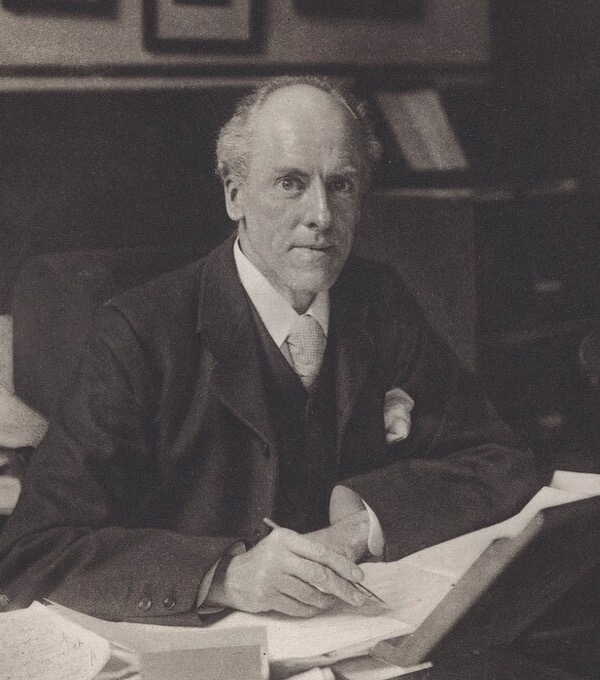
\includegraphics[width=\linewidth]{karl-pearson.jpg}\\
      {\scriptsize\color{gray}En 1910. Domaine public, National Portrait
      Gallery (Londres), Wikimedia Commons.}
    \end{column}
    \begin{column}{0.72\textwidth}
      \begin{itemize}
        \item Né à Londres ; mathématiques à Cambridge, puis physique,
          philosophie et droit en Allemagne. En 1884, professeur de
          mathématiques appliquées à l'University College de Londres.
        \item Sous l'influence de Galton et de Weldon, il se tourne vers
          l'étude statistique de l'hérédité et de l'évolution : la
          biométrie.
        \item L'un des fondateurs de la statistique moderne : l'expression
          « écart type », le coefficient de corrélation, le test du
          khi-deux, la revue Biometrika (1901).
        \item 1901 : « Sur les lignes et les plans qui s'ajustent au plus près
          à des systèmes de points de l'espace ».
      \end{itemize}
    \end{column}
  \end{columns}
\end{frame}

\begin{frame}{Note historique 5.1 (suite)}
  \small
  \begin{itemize}
    \item Pearson remarque que les deux droites de régression dépendent de
      la variable que l'on choisit d'expliquer.
    \item Il propose de minimiser la somme des carrés des distances
      perpendiculaires : exactement le problème de la section 2.
    \item Il montre que cette droite passe par le centre de gravité et
      qu'elle est portée par le grand axe de l'« ellipsoïde de corrélation »
      --- un vecteur propre de la matrice de covariance.
    \item Comme Galton, il fut un ardent défenseur de l'eugénisme ; en 1911,
      premier titulaire de la chaire d'eugénisme créée par le testament de
      Galton. Ces idées, qui ont servi à justifier des stérilisations
      forcées au \siecle{20}, sont aujourd'hui unanimement rejetées ; en
      2020, l'University College a retiré leurs noms de plusieurs
      bâtiments.
    \item Des outils mathématiques solides peuvent être mis au service de
      projets condamnables.
  \end{itemize}
\end{frame}

\begin{frame}{Hotelling, Spearman et la suite}
  \small
  \begin{itemize}
    \item Harold Hotelling (1895--1973) redécouvre la méthode et lui donne
      son nom (1933) : « Analyse d'un ensemble de variables statistiques en
      composantes principales », dans le Journal of Educational Psychology,
      sur des résultats d'élèves en lecture et en arithmétique.
    \item Le contexte : Spearman (1904) avait observé que les notes
      d'écoliers dans toutes les matières sont corrélées positivement, et en
      avait déduit un facteur général d'intelligence, $g$. Nos six élèves,
      dont l'axe principal mesure le « niveau général », en sont un écho
      lointain.
    \item Hotelling propose une méthode itérative de calcul, voisine de la
      méthode des puissances du chapitre 4.
    \item Longtemps limitée par le calcul (une matrice $10\times10$ à la
      main : plusieurs jours de travail), l'ACP se répand avec les
      ordinateurs. En France, l'école d'« analyse des données » de
      Jean-Paul Benzécri (années 1960--1970).
    \item Autres noms : la transformation de Karhunen--Loève en traitement du
      signal. Aujourd'hui, l'une des méthodes les plus employées de la
      statistique.
  \end{itemize}
\end{frame}

% ═══════════════════════════════════════════════════════════════════════
\section{Au-delà de trois dimensions}
% ═══════════════════════════════════════════════════════════════════════

\begin{frame}{Le décathlon}
  \small
  \begin{itemize}
    \item Dix épreuves sur deux jours : quatre courses ($100$ m, $400$ m,
      $110$ m haies, $1500$ m), trois sauts (longueur, hauteur, perche),
      trois lancers (poids, disque, javelot).
    \item $41$ résultats de 2004 : Décastar de Talence et Jeux olympiques
      d'Athènes. Chaque résultat est un point de $\R^{10}$ ; aucun dessin
      direct n'est possible.
  \end{itemize}
  \scriptsize Tableau 5.3 --- Quelques décathloniens en 2004 (secondes pour les
  courses, mètres pour les sauts et les lancers).
  \begin{center}
    \scriptsize
    \setlength{\tabcolsep}{4pt}
    \begin{tabular}{lcccccccccc}
      \toprule
      Athlète & $100$ & Long. & Poids & Haut. & $400$ & Haies & Disque & Perche & Jav. & $1500$ \\
      \midrule
      Sebrle & $\num{10.85}$ & $\num{7.84}$ & $\num{16.36}$ & $\num{2.12}$ & $\num{48.36}$ & $\num{14.05}$ & $\num{48.72}$ & $\num{5.00}$ & $\num{70.52}$ & $\num{280.01}$ \\
      Karpov & $\num{10.50}$ & $\num{7.81}$ & $\num{15.93}$ & $\num{2.09}$ & $\num{46.81}$ & $\num{13.97}$ & $\num{51.65}$ & $\num{4.60}$ & $\num{55.54}$ & $\num{278.11}$ \\
      Drews & $\num{10.87}$ & $\num{7.38}$ & $\num{13.07}$ & $\num{1.88}$ & $\num{48.51}$ & $\num{14.01}$ & $\num{40.11}$ & $\num{5.00}$ & $\num{51.53}$ & $\num{274.21}$ \\
      Casarsa & $\num{11.36}$ & $\num{6.68}$ & $\num{14.92}$ & $\num{1.94}$ & $\num{53.20}$ & $\num{15.39}$ & $\num{48.66}$ & $\num{4.40}$ & $\num{58.62}$ & $\num{296.12}$ \\
      \midrule
      moyenne & $\num{11.00}$ & $\num{7.26}$ & $\num{14.48}$ & $\num{1.98}$ & $\num{49.62}$ & $\num{14.61}$ & $\num{44.33}$ & $\num{4.76}$ & $\num{58.32}$ & $\num{279.02}$ \\
      \bottomrule
    \end{tabular}
  \end{center}
  \small Unités et dispersions différentes : on réduit ; la variance totale
  vaut $10$.
\end{frame}

\begin{frame}[fragile]{Programme 5.3 --- L'ACP du décathlon}
\begin{lstlisting}
deca = pd.read_csv("decathlon.csv", index_col=0)
X = deca.iloc[:, :10].to_numpy()        # les dix épreuves
valeurs, vecteurs, Y = acp(X)
print("valeurs propres :", valeurs.round(2))
print("% cumulés :", (100 * np.cumsum(valeurs) / valeurs.sum()).round(1))
r = np.corrcoef(Y[:, 0], deca["Points"])[0, 1]
print("corrélation y1 / points :", round(r, 3))
\end{lstlisting}
  \vspace{4pt}
  \small Sortie (la fonction \texttt{acp} est celle du programme 5.1) :
  \begin{center}
    \footnotesize
    \begin{tabular}{lcccccccccc}
      \toprule
      $k$ & $1$ & $2$ & $3$ & $4$ & $5$ & $6$ & $7$ & $8$ & $9$ & $10$ \\
      \midrule
      $\lambda_k$ & $\num{3.27}$ & $\num{1.74}$ & $\num{1.40}$ & $\num{1.06}$ & $\num{0.68}$ & $\num{0.60}$ & $\num{0.45}$ & $\num{0.40}$ & $\num{0.21}$ & $\num{0.18}$ \\
      \% cumulé & $\num{32.7}$ & $\num{50.1}$ & $\num{64.1}$ & $\num{74.7}$ & $\num{81.6}$ & $\num{87.5}$ & $\num{92.1}$ & $\num{96.0}$ & $\num{98.2}$ & $100$ \\
      \bottomrule
    \end{tabular}
  \end{center}
  Corrélation entre $y_1$ et le total officiel des points : $\num{0.956}$.
\end{frame}

\begin{frame}{Figure 5.9 --- Le diagramme des éboulis}
  \begin{columns}[c]
    \begin{column}{0.55\textwidth}
      \FigLivre[0.62\textheight]{fig-acp-eboulis}
      \scriptsize La droite pointillée : le seuil du critère de Kaiser.
    \end{column}
    \begin{column}{0.43\textwidth}
      \small
      \begin{itemize}
        \item Beaucoup moins tranché que pour les manchots : le plan
          principal ne conserve qu'environ la moitié de l'information
          ($\SI{32.7}{\percent}+\SI{17.4}{\percent}$).
        \item Kaiser retiendrait quatre axes ; il en faudrait cinq pour
          dépasser $\SI{80}{\percent}$.
        \item Pas un échec : une information sur les données. Les dix
          épreuves sont assez indépendantes ; on ne résume pas un
          décathlonien par deux nombres.
      \end{itemize}
    \end{column}
  \end{columns}
\end{frame}

\begin{frame}{Lire le plan principal}
  \begin{columns}[c]
    \begin{column}{0.4\textwidth}
      \scriptsize Tableau 5.4 --- Les deux premiers vecteurs propres.
      \begin{center}
        \scriptsize
        \begin{tabular}{lcc}
          \toprule
          Épreuve & $\vec v_1$ & $\vec v_2$ \\
          \midrule
          $100$ m & $-\num{0.428}$ & $\num{0.142}$ \\
          saut en longueur & $\num{0.410}$ & $-\num{0.262}$ \\
          lancer du poids & $\num{0.344}$ & $\num{0.454}$ \\
          saut en hauteur & $\num{0.316}$ & $\num{0.266}$ \\
          $400$ m & $-\num{0.376}$ & $\num{0.432}$ \\
          $110$ m haies & $-\num{0.413}$ & $\num{0.174}$ \\
          lancer du disque & $\num{0.305}$ & $\num{0.460}$ \\
          saut à la perche & $\num{0.028}$ & $-\num{0.137}$ \\
          lancer du javelot & $\num{0.153}$ & $\num{0.241}$ \\
          $1500$ m & $-\num{0.032}$ & $\num{0.360}$ \\
          \bottomrule
        \end{tabular}
      \end{center}
    \end{column}
    \begin{column}{0.58\textwidth}
      \small
      \begin{itemize}
        \item Premier axe : vitesse ($100$ m, haies, $400$ m) négative, saut
          en longueur positif. Un bon temps est un temps court : à droite,
          les athlètes qui courent vite et sautent loin. La performance
          générale.
        \item Second axe : les lancers (poids, disque), mais aussi le $400$ m
          et le $1500$ m. En haut : puissants, mais relativement lents sur
          les courses longues (Casarsa : disque à $\num{48.66}$ m,
          $400$ m en $\num{53.20}$ s).
        \item La perche, aux deux composantes faibles, est mal représentée :
          c'est le troisième axe qui la décrit.
      \end{itemize}
    \end{column}
  \end{columns}
\end{frame}

\begin{frame}{Figure 5.10 --- Les athlètes dans le plan principal}
  \begin{columns}[c]
    \begin{column}{0.58\textwidth}
      \FigLivre[0.72\textheight]{fig-acp-decathlon}
    \end{column}
    \begin{column}{0.4\textwidth}
      \small
      \begin{itemize}
        \item La première composante a été calculée sans le barème officiel,
          qui convertit chaque performance en points selon des tables
          complexes.
        \item Pourtant, sa corrélation avec le total des points vaut
          $\num{0.956}$ : les trois médaillés d'Athènes, Sebrle, Clay et
          Karpov, sont les trois points les plus à droite.
        \item L'ACP a retrouvé seule ce que signifie « être un bon
          décathlonien ».
      \end{itemize}
    \end{column}
  \end{columns}
\end{frame}

\begin{frame}{D'autres applications}
  \begin{itemize}
    \item Génétique : Novembre et ses collègues (2008), près de
      $\num{1400}$ Européens décrits par environ $\num{200000}$ marqueurs.
      Dans le plan principal, convenablement tourné, le nuage reproduit la
      carte de l'Europe.
    \item Images : une photo de $100\times100$ pixels est un point de
      $\R^{\num{10000}}$. Les vecteurs propres d'un grand nombre de visages
      sont des « visages propres » (eigenfaces) ; quelques dizaines de
      coordonnées suffisent à bien décrire un visage.
    \item Compresser des données, éliminer du bruit, réduire le nombre de
      variables avant une autre méthode d'apprentissage automatique.
    \item Souvent la première chose que l'on fait devant un nouveau jeu de
      données.
  \end{itemize}
\end{frame}

\begin{frame}{Les limites de la méthode}
  \begin{itemize}
    \item L'ACP est linéaire : elle cherche des droites et des plans, et
      passe à côté d'une structure courbe (un nuage le long d'un arc de
      cercle).
    \item Elle est sensible aux unités (remarque 5.4) et aux valeurs
      aberrantes, qui peuvent accaparer un axe à elles seules :
      \begin{itemize}
        \item deux élèves atypiques ajoutés aux six font passer la
          corrélation de $\num{0.8}$ à environ $-\num{0.08}$ et basculer
          l'axe principal (exercice 5.5) ;
        \item une masse de manchot saisie à $\num{42000}$ g au lieu de
          $\num{4200}$ g s'empare du deuxième axe, même après réduction
          (exercice 5.10).
      \end{itemize}
      Avant d'interpréter : regarder les données et repérer les individus
      atypiques.
    \item Une grande variance n'est pas toujours une information
      intéressante : la direction qui sépare deux groupes peut être une
      direction de faible variance.
  \end{itemize}
\end{frame}

\begin{frame}{Pour la classe 5.4 --- Des données réelles en classe}
  \begin{Classe}{Des données réelles en classe}
    \small
    \begin{itemize}
      \item Le programme insiste sur l'interprétation de données et le regard
        critique sur l'information statistique.
      \item Sans algèbre linéaire : distribuer les mesures d'une cinquantaine
        de manchots, sans l'espèce. Quel nuage de points, pour quelle paire
        de variables, montre le mieux qu'il y a « plusieurs sortes » de
        manchots ?
      \item L'idée centrale du chapitre : un même ensemble de données,
        regardé sous différents angles, peut révéler ou cacher sa structure.
      \item Élèves plus avancés : un tableur pour calculer les cotes $z$, et
        constater que les variables réduites deviennent comparables.
      \item Construire un « score » combinant plusieurs épreuves d'éducation
        physique, et le comparer à une simple somme des cotes $z$.
    \end{itemize}
  \end{Classe}
\end{frame}

% ═══════════════════════════════════════════════════════════════════════
\section{Synthèse}
% ═══════════════════════════════════════════════════════════════════════

\begin{frame}{Ce qu'il faut retenir}
  \small
  \begin{itemize}
    \item Un tableau de données est un nuage de points ; on ne le voit
      qu'en projection.
    \item Pythagore : minimiser les distances au sous-espace revient à
      maximiser la variance du nuage projeté.
    \item La variance dans la direction $\vec u$ est $\vec u^{\mathsf T}C\,\vec u$ ;
      ses extremums sont dans les directions propres de la matrice de
      covariance $C$, et valent les valeurs propres.
    \item ACP : diagonaliser $C$ (théorème spectral), ranger
      $\lambda_1\geq\dots\geq\lambda_p$, projeter sur
      $\vec v_1,\dots,\vec v_q$ ; les composantes principales sont non
      corrélées, de variances $\lambda_k$.
    \item La proportion $\frac{\lambda_1+\dots+\lambda_q}{\lambda_1+\dots+\lambda_p}$
      dit jusqu'à quel point le dessin est fidèle ; l'erreur de
      reconstruction moyenne est $\lambda_{q+1}+\dots+\lambda_p$.
    \item Réduire (matrice de corrélation) dès que les unités ou les
      ordres de grandeur diffèrent ; se méfier des valeurs aberrantes.
    \item Interpréter les axes à l'aide des composantes des vecteurs
      propres : « niveau général », « taille du bec », « performance ».
  \end{itemize}
\end{frame}

\begin{frame}{Des notions du secondaire aux applications modernes}
  \small
  \begin{center}
  \begin{tabular}{ll}
    \toprule
    Notion du secondaire & Rôle dans l'ACP \\
    \midrule
    nuage de points, corrélation & le point de départ ; la forme du nuage \\
    droite de régression & un point de comparaison avec l'axe principal \\
    cote $z$ & réduire les variables \\
    fonction sinusoïdale & la variance selon l'angle d'une droite \\
    vecteurs, produit scalaire & projeter \\
    théorème de Pythagore & l'équivalence des deux problèmes \\
    \bottomrule
  \end{tabular}
  \end{center}
  \vspace{6pt}
  Une méthode de 1901, devenue l'un des outils les plus employés de la
  statistique et de la science des données : le calcul de quelques vecteurs
  propres d'une matrice symétrique.
\end{frame}

\begin{frame}{Et maintenant}
  \begin{itemize}
    \item Les démonstrations laissées « au tableau » sont toutes dans les
      notes de cours, avec tous les détails.
    \item Exercices du chapitre (avec solutions complètes) : calculs à la
      main (5.1 à 5.6), dont les valeurs extrêmes (5.5) ; programmes Python
      (5.7 à 5.11), dont l'erreur de saisie (5.10) ; réflexion pour la
      classe (5.12).
    \item L'application interactive des manchots est sur le site des notes :
      \href{\urlappli}{\color{sectioncolor}ouvrir l'application}.
    \item Les rappels d'algèbre linéaire (projection orthogonale, valeurs
      propres, théorème spectral) sont à l'annexe D.
  \end{itemize}
\end{frame}


\end{document}
